\documentclass[a4paper,11pt]{article}
\usepackage{sbpo-template}
\usepackage[brazil]{babel}
\usepackage[utf8]{inputenc}
\usepackage[T1]{fontenc}
\usepackage{amsmath,amssymb,bm,icomma}
\usepackage{url}
\usepackage{graphicx}
\usepackage{booktabs}
\usepackage[table]{xcolor}
\usepackage[square]{natbib}
\usepackage{indentfirst}

\definecolor{fundo}{HTML}{EAF1F7}
\graphicspath{{figuras/}}
\newcommand{\nGiniCorUF}{0,995}
\newcommand{\nGiniDifUF}{0,008}
\newcommand{\nHomAno}{46.105}
\newcommand{\nTaxaNbr}{36,4}
\newcommand{\nTaxaNEbr}{36,9}
\newcommand{\nTaxaSEbr}{13,0}
\newcommand{\nTaxaCObr}{22,2}
\newcommand{\nTaxaSbr}{16,7}
\newcommand{\nTaxaBR}{22,7}
\newcommand{\nPctIntervencao}{4,7}
\newcommand{\nTaxaBrasilContexto}{21,3}
\newcommand{\nTaxaMundoContexto}{5,8}
\newcommand{\nPopMin}{30}
\newcommand{\nMunCorte}{1.134}
\newcommand{\nPercCorte}{80}
\newcommand{\nCasosEspCorte}{20}
\newcommand{\nOscCorte}{22}
\newcommand{\nForaNome}{Campos do Jordão-SP}
\newcommand{\nForaHom}{1}
\newcommand{\nForaIndet}{36}
\newcommand{\nMunEsc}{1.133}
\newcommand{\nPctPopEsc}{77}
\newcommand{\nPctHomEsc}{78}
\newcommand{\nMunFora}{4.437}
\newcommand{\nTaxaFora}{22,1}
\newcommand{\nTaxaEsc}{22,9}
\newcommand{\nMunZeroHom}{655}
\newcommand{\nMunSemEM}{7}
\newcommand{\nCorUrbana}{$-$0,23}
\newcommand{\nCorDesocup}{$+$0,30}
\newcommand{\nCorRendaUrbana}{0,74}
\newcommand{\nCorQuadSem}{0,999}
\newcommand{\nCentroRenda}{1.255}
\newcommand{\nCentroGini}{0,463}
\newcommand{\nLambdaFinal}{0,17}
\newcommand{\nLambdaFinalInf}{0,12}
\newcommand{\nLambdaFinalSup}{0,23}
\newcommand{\nSWy}{0,930}
\newcommand{\nSWln}{0,998}
\newcommand{\nBPlambda}{26,7}
\newcommand{\nGiniEfD}{16,2}
\newcommand{\nPDesD}{0,182}
\newcommand{\nPDesFinal}{0,022}
\newcommand{\nPressPred}{0,552}
\newcommand{\nRdoisAC}{0,431}
\newcommand{\nRdoisAD}{0,533}
\newcommand{\nFUltMin}{31,1}
\newcommand{\nFUltMax}{64,6}
\newcommand{\nRdoisE}{0,564}
\newcommand{\nRdoisA}{0,558}
\newcommand{\nRdoisPct}{56}
\newcommand{\nFglobal}{111}
\newcommand{\nGlUm}{13}
\newcommand{\nGlDois}{1.119}
\newcommand{\nEfFreq}{8,6}
\newcommand{\nEfDist}{15,6}
\newcommand{\nEfUrb}{11,8}
\newcommand{\nEfMigr}{2,1}
\newcommand{\nEfDesoc}{1,8}
\newcommand{\nPMigr}{0,143}
\newcommand{\nGiniEfMediana}{15,8}
\newcommand{\nGiniEfNoventa}{33,7}
\newcommand{\nGiniEfDez}{10,0}
\newcommand{\nGiniPDez}{0,008}
\newcommand{\nRendaDez}{699}
\newcommand{\nRendaMediana}{1.383}
\newcommand{\nRendaNoventa}{2.043}
\newcommand{\nGiniZero}{931}
\newcommand{\nGiniZeroPct}{29}
\newcommand{\nPico}{815}
\newcommand{\nPctAbaixoPico}{20}
\newcommand{\nNAbaixoPico}{224}
\newcommand{\nNAbaixoPicoNNE}{222}
\newcommand{\nIqrGini}{0,051}
\newcommand{\nPctNEpobres}{63}
\newcommand{\nPctNpobres}{37}
\newcommand{\nEfNordeste}{108}
\newcommand{\nIcInfNordeste}{84}
\newcommand{\nIcSupNordeste}{134}
\newcommand{\nEfCentroOeste}{83}
\newcommand{\nIcInfCentroOeste}{59}
\newcommand{\nIcSupCentroOeste}{110}
\newcommand{\nEfNorte}{79}
\newcommand{\nIcInfNorte}{52}
\newcommand{\nIcSupNorte}{110}
\newcommand{\nEfSul}{67}
\newcommand{\nIcInfSul}{50}
\newcommand{\nIcSupSul}{86}
\newcommand{\nUFpoucos}{5}
\newcommand{\nPDesRenda}{0,218}
\newcommand{\nPDesGini}{0,106}
\newcommand{\nRdoisATodos}{0,572}
\newcommand{\nPRegGini}{0,278}
\newcommand{\nBICfinal}{1.381}
\newcommand{\nBICtodos}{1.343}
\newcommand{\nBICcubo}{1.382}
\newcommand{\nCpFinal}{48}
\newcommand{\nPmaisUm}{14}
\newcommand{\nEfNordesteRR}{82}
\newcommand{\nEfSulRR}{37}
\newcommand{\nVIFrendaFinal}{7,6}
\newcommand{\nVIFmedio}{2,4}
\newcommand{\nVIFgini}{1,8}
\newcommand{\nVIFdesoc}{2,1}
\newcommand{\nVIFquad}{1,5}
\newcommand{\nRdoisRenda}{87}
\newcommand{\nBP}{46,0}
\newcommand{\nBPgl}{13}
\newcommand{\nSW}{0,998}
\newcommand{\nSWp}{0,165}
\newcommand{\nMaxSemi}{3,9}
\newcommand{\nSigma}{0,524}
\newcommand{\nFatorDoisS}{2,85}
\newcommand{\nBPpop}{5,6}
\newcommand{\nBPpopP}{0,018}
\newcommand{\nRegraUm}{69,4}
\newcommand{\nRegraDois}{90,7}
\newcommand{\nRegraTres}{94,7}
\newcommand{\nVarAjMenor}{0,34}
\newcommand{\nVarAjMaior}{0,16}
\newcommand{\nBPaj}{27,7}
\newcommand{\nSzeroQ}{0,239}
\newcommand{\nMqpInter}{7,328}
\newcommand{\nMqoInter}{7,398}
\newcommand{\nEpMin}{0,97}
\newcommand{\nEpMax}{1,00}
\newcommand{\nBPmqp}{32,0}
\newcommand{\nBPmqpP}{0,002}
\newcommand{\nBPmqpPop}{0,9}
\newcommand{\nBPmqpPopP}{0,341}
\newcommand{\nBPmqpAj}{15,1}
\newcommand{\nNSensDesoc}{31}
\newcommand{\nRazIndetMax}{12}
\newcommand{\nPSensDesoc}{0,072}
\newcommand{\nSemiCJ}{$-$4,9}
\newcommand{\nInterCJ}{7,453}
\newcommand{\nEfSulSemSP}{27}
\newcommand{\nRdoisResUF}{17}
\newcommand{\nFResUF}{8,5}
\newcommand{\nGlResUFa}{26}
\newcommand{\nGlResUFb}{1.106}
\newcommand{\nGiniEfDUF}{6,2}
\newcommand{\nGiniPDUF}{0,011}
\newcommand{\nRdoisAUF}{0,638}
\newcommand{\nBICUF}{1.473}
\newcommand{\nAICUF}{1.654}
\newcommand{\nAICfinalUF}{1.451}
\newcommand{\nPMigrUF}{0,064}
\newcommand{\nPDezMin}{5,9}
\newcommand{\nPDezMax}{12,1}
\newcommand{\nPDezSig}{6}
\newcommand{\nNEspec}{8}
\newcommand{\nTodosMed}{10,8}
\newcommand{\nUFFracMed}{41}
\newcommand{\nUFFracNov}{53}
\newcommand{\nPMigrVinte}{0,002}
\newcommand{\nPMigrVinteCinco}{0,040}
\newcommand{\nGiniDCorteMin}{11,5}
\newcommand{\nGiniDCorteMax}{16,3}
\newcommand{\nHRefMax}{0,003}
\newcommand{\nHMedia}{0,012}

\newcommand{\fonte}{Fonte: elaboração própria com dados do SIM/DATASUS, do IBGE e do INEP.}

\title{FATORES ASSOCIADOS AOS HOMICÍDIOS NOS MUNICÍPIOS BRASILEIROS}

\begin{document}

\maketitle

\author{
\name{Douglas Bergamim Fernandes}
\email{douglas.fernandes.8912@ga.ita.br}
}

\author{
\name{Fabio Eiiti Kobayashi Urio}
\email{fabio.urio.8913@ga.ita.br}
}

\author{
\name{Kauan Alves Aragão}
\email{kauan.aragao.9012@ga.ita.br}
}

\author{
\name{Luiz Felipe de Brito Ramos}
\email{luiz.ramos.8892@ga.ita.br}
}

\author{
\name{Willian Nelton Teleken}
\email{willian.teleken.8968@ga.ita.br}
}

{
\vspace{6pt}
\institute{Instituto Tecnológico de Aeronáutica (ITA)}
\iaddress{Praça Marechal Eduardo Gomes, 50, Vila das Acácias, São José dos Campos -- SP}
}

\vspace{8mm}
\begin{resumo}
Ligado ao ODS 16, este trabalho investiga quais características socioeconômicas, demográficas e geográficas estão associadas à taxa de homicídios dos municípios brasileiros. Usamos os óbitos por agressão e intervenção legal do SIM (média de 2021--2023), o Censo 2022 e dados do INEP para os \nMunEsc{} municípios com 30 mil habitantes ou mais. Ajustamos uma regressão linear múltipla para o logaritmo da taxa, com renda quadrática, índice de Gini, interação Gini--renda, desocupação, urbanização, frequência e atraso escolar, migração recente e região. O modelo explica \nRdoisPct\% da variação do logaritmo da taxa. A associação da desigualdade depende da renda: é positiva nos municípios de renda média e alta. Mais frequência e menos atraso escolar associam-se a taxas menores. A migração não mostrou associação clara. A variância dos erros não é constante; os resultados são associações.
\end{resumo}

\bigskip
\begin{palchaves}
Homicídios. Municípios brasileiros. Regressão linear múltipla. Desigualdade.
\end{palchaves}

\vspace{8mm}

\begin{abstract}
Linked to SDG 16, this work investigates which socioeconomic, demographic and geographic characteristics are associated with the homicide rate of Brazilian municipalities. We use deaths from assault and legal intervention from the Mortality Information System (2021--2023 average), the 2022 Census and INEP data for the 1,133 municipalities with 30,000 inhabitants or more. We fit a multiple linear regression for the logarithm of the rate, with quadratic income, the Gini index, a Gini-income interaction, unemployment, urbanization, school attendance and age-grade distortion, recent migration and region. The model explains 56\% of the variation of the log rate. The association of inequality depends on income: it is positive in middle- and high-income municipalities. Higher school attendance and lower age-grade distortion are associated with lower rates. Recent migration showed no clear association. The error variance is not constant; the results are associations.
\end{abstract}

\bigskip
\begin{keywords}
Homicides. Brazilian municipalities. Multiple linear regression. Inequality.
\end{keywords}

\newpage

\section{Introdução}

Os Objetivos de Desenvolvimento Sustentável (ODS) são dezessete objetivos da ONU para a Agenda 2030. O ODS 16, Paz, Justiça e Instituições Eficazes, tem como meta 16.1 reduzir significativamente todas as formas de violência e as taxas de mortalidade relacionadas. O indicador 16.1.1 mede as vítimas de homicídio intencional por 100 mil habitantes \citep{onu2025metadados}.

O Brasil está longe dessa meta. Em 2021, a taxa brasileira foi de \nTaxaBrasilContexto{} homicídios intencionais por 100 mil habitantes, contra \nTaxaMundoContexto{} no mundo \citep{unodc2023}. Na base deste trabalho, o país registrou em média \nHomAno{} mortes por agressão ou intervenção legal por ano entre 2021 e 2023. As taxas também variam muito dentro do país (Figura~\ref{fig:mapa}). Considerando todos os municípios, a taxa anual foi de \nTaxaNEbr{} por 100 mil no Nordeste, \nTaxaNbr{} no Norte, \nTaxaCObr{} no Centro-Oeste, \nTaxaSbr{} no Sul e \nTaxaSEbr{} no Sudeste.

A literatura associa a violência letal a condições econômicas e sociais. Em painéis de países, a desigualdade de renda associa-se a taxas maiores de crimes violentos \citep{fajnzylber2002}; em condados urbanos dos Estados Unidos, a desigualdade tem efeito forte sobre o crime violento e nenhum sobre o crime contra o patrimônio \citep{kelly2000}. Esse efeito, porém, pode perder força quando se controlam diferenças fixas entre países \citep{neumayer2003}. A relação com a renda também não parece linear: o crime acompanha a renda em forma de U invertido \citep{buonanno2017}, e, nos municípios brasileiros, o risco de homicídio de homens adultos foi maior nas categorias intermediárias de renda \citep{duarte2012}. Há indícios de que renda e desigualdade interagem: a desigualdade prediz o homicídio sobretudo em países de desenvolvimento médio \citep{ouimet2012} e condiciona o efeito do PIB sobre os homicídios em países desenvolvidos \citep{aransiola2024}.

No Brasil, um estudo com os 5.570 municípios encontrou risco maior com mais urbanização, mais população e maior índice de Gini \citep{wanzinack2022}, mas estimou um único efeito do Gini para todos os municípios. Uma revisão sistemática aponta a educação como possível fator de proteção \citep{wanzinack2018}, e um estudo com estados estimou que mais gasto em educação reduz a taxa de homicídios no período seguinte \citep{becker2017}. A teoria da desorganização social relaciona a mobilidade residencial e a fragilidade dos laços comunitários ao crime \citep{sampson1989}; no Brasil, a desorganização social associou-se a trajetórias crescentes de homicídio entre 1991 e 2010 \citep{peres2017}. Este trabalho testa, entre municípios brasileiros, se a associação da desigualdade muda com a renda.

\begin{figure}[htbp]
\centering
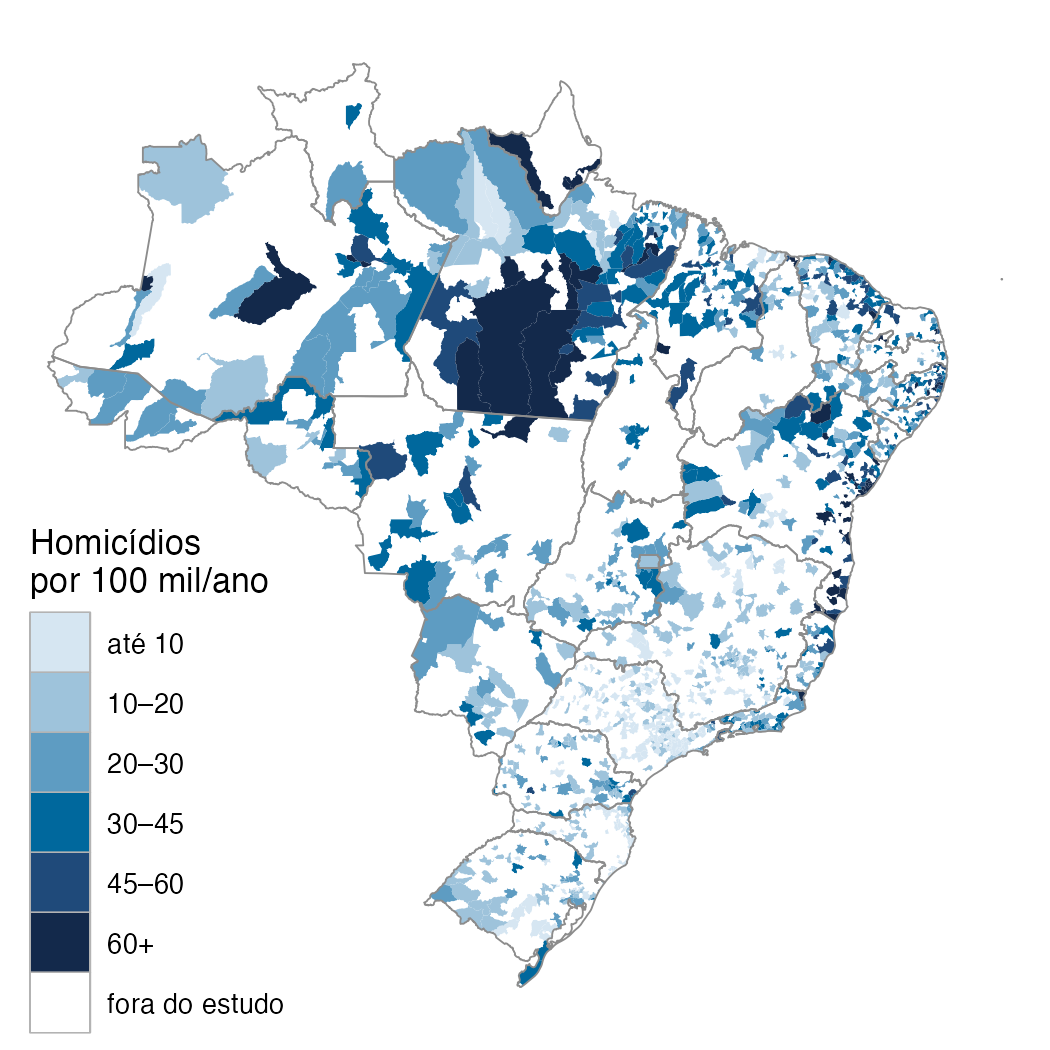
\includegraphics[width=0.50\textwidth]{mapa_taxa.png}
\caption{Taxa de homicídios por 100 mil habitantes ao ano, 2021--2023, nos municípios do estudo. Em cinza, os municípios fora do escopo: menos de 30 mil habitantes e Campos do Jordão-SP. Fonte: elaboração própria com dados do SIM/DATASUS e do IBGE.}
\label{fig:mapa}
\end{figure}

\subsection{Questão de Pesquisa}

Quais características socioeconômicas, demográficas e geográficas estão associadas à taxa de homicídios nos municípios brasileiros? Em particular, a associação da desigualdade com a taxa muda conforme a renda do município?

Com base na literatura, o grupo formulou três hipóteses antes de ajustar o modelo. \textbf{H1}: municípios mais desiguais têm taxas maiores \citep{fajnzylber2002, kelly2000}. \textbf{H2}: municípios com mais exclusão escolar de jovens têm taxas maiores \citep{wanzinack2018, becker2017}. \textbf{H3}: municípios com mais migração recente, um componente da mobilidade residencial, têm taxas maiores \citep{sampson1989, peres2017}. Ao final, cada hipótese é classificada como sustentada, parcialmente sustentada ou não sustentada.

\subsection{Objetivos}

\textbf{Objetivo Geral:} identificar as características municipais associadas à taxa de homicídios por meio de um modelo de regressão linear múltipla.

\textbf{Objetivos Específicos:}
\begin{itemize}
\item montar uma base municipal com dados de mortalidade, do Censo 2022 e de indicadores educacionais;
\item ajustar e diagnosticar um modelo de regressão linear múltipla para o logaritmo da taxa de homicídios;
\item testar se a associação da desigualdade depende da renda do município;
\item avaliar as hipóteses H1, H2 e H3 e discutir as limitações do modelo.
\end{itemize}

\section{Metodologia}

\subsection{Base de dados}

A unidade de análise é o município, e o estudo é observacional. A variável resposta é a taxa anual de homicídios por 100 mil habitantes:
\[
Y_i = \frac{\text{óbitos em 2021--2023}}{3 \times \text{população de 2022}} \times 100\,000.
\]
Os óbitos foram obtidos do Sistema de Informações sobre Mortalidade (SIM), por município de residência \citep{datasus2025}. Somamos as agressões (CID-10 X85--Y09) e as intervenções legais e operações de guerra (Y35--Y36). Essa medida se relaciona ao indicador 16.1.1, mas não replica a sua definição internacional. A média de três anos reduz a oscilação de um ano isolado.

As variáveis explicativas vêm do Censo Demográfico 2022 \citep{ibge2023censo} e dos Indicadores Educacionais 2022 do INEP \citep{inep2023}:
\begin{itemize}
\item \textbf{renda}: rendimento domiciliar per capita médio, em logaritmo;
\item \textbf{desigualdade}: índice de Gini do rendimento domiciliar per capita, calculado sobre as pessoas de 14 anos ou mais;
\item \textbf{desocupação}: percentual da força de trabalho sem ocupação;
\item \textbf{urbanização}: percentual da população em situação urbana;
\item \textbf{frequência escolar}: taxa de frequência escolar bruta de 15 a 17 anos;
\item \textbf{distorção idade-série}: percentual de alunos do ensino médio com dois anos ou mais de atraso escolar;
\item \textbf{migração recente}: percentual de moradores que residem no município há menos de dez anos;
\item \textbf{região}: Norte, Nordeste, Centro-Oeste, Sudeste e Sul, com o Sudeste como referência.
\end{itemize}

O IBGE não publica o Gini municipal do Censo 2022. O Censo publica, por município, o número de pessoas de 14 anos ou mais em cada classe de rendimento domiciliar per capita. Calculamos o índice por essas classes, pelo método de \citet{gastwirth1972}: cada classe recebe o ponto médio da sua faixa, e o Gini é 1 menos o dobro da área sob a curva de Lorenz. A classe aberta (mais de 20 salários mínimos) recebe 50 salários mínimos, valor com que o cálculo reproduz o Gini oficial do Brasil; esse valor foi escolhido no total do país, e não em cada UF. Nas 27 UFs, o Gini calculado tem correlação de \nGiniCorUF{} com o oficial, e a maior diferença é de \nGiniDifUF. O cálculo do Gini por município veio da revisão da professora e não está descrito na apostila.

\textbf{Recorte.} Em municípios pequenos, poucas mortes mudam muito a taxa. Por isso, o estudo usa os municípios com \nPopMin{} mil habitantes ou mais. O corte fica perto do percentil \nPercCorte{} da população municipal; o uso de um percentil como corte também veio da revisão da professora. Com a taxa nacional da base (\nTaxaBR{} por 100 mil), esse porte corresponde a cerca de \nCasosEspCorte{} homicídios esperados em três anos. Excluímos \nForaNome{} por indício de sub-registro: \nForaHom{} homicídio registrado e \nForaIndet{} óbitos de intenção indeterminada em três anos. Restam \nMunEsc{} municípios, com \nPctPopEsc\% da população do país. A Tabela~\ref{tab:descritiva} resume as variáveis, e a Tabela~\ref{tab:cor} mostra a correlação simples de cada explicativa com o logaritmo da taxa.

\begin{table}[htbp]
\centering
\caption{Estatísticas descritivas dos \nMunEsc{} municípios do estudo. \fonte}
\label{tab:descritiva}
\small
\begin{tabular}{@{}lrrrrrr@{}}
\toprule
\textbf{Variável} & \textbf{Média} & \textbf{DP} & \textbf{Mín.} & \textbf{Mediana} & \textbf{Máx.} & \textbf{Cor.}\\
\midrule
Taxa de homicídios (/100 mil/ano) & 24,7 & 17,8 & 1,0 & 20,4 & 116,0 & ---\\
Renda \textit{per capita} (R\$/mês) & 1.368 & 559 & 359 & 1.383 & 4.300 & $-$0,48\\
Desigualdade (índice de Gini) & 0,463 & 0,043 & 0,325 & 0,463 & 0,652 & 0,26\\
Desocupação (\%) & 5,7 & 2,8 & 1,0 & 5,2 & 21,0 & 0,30\\
Urbanização (\%) & 83,9 & 16,9 & 22,2 & 90,9 & 100,0 & $-$0,23\\
Frequência escolar 15--17 (\%) & 85,3 & 4,5 & 64,0 & 85,8 & 96,4 & $-$0,16\\
Distorção idade-série EM (\%) & 22,9 & 12,0 & 2,6 & 20,4 & 66,6 & 0,49\\
Migração recente (\%) & 15,5 & 6,6 & 3,3 & 13,9 & 53,0 & $-$0,04\\
\bottomrule
\end{tabular}

\end{table}

\begin{table}[htbp]
\centering
\caption{Correlação simples de cada explicativa com ln(taxa), nos \nMunEsc{} municípios. \fonte}
\label{tab:cor}
\footnotesize
\setlength{\tabcolsep}{3pt}
\begin{tabular}{@{}lrrrrrrr@{}}
\toprule
 & \textbf{ln(renda)} & \textbf{Gini} & \textbf{Desocupação} & \textbf{Urbana} & \textbf{Freq. escolar} & \textbf{Distorção EM} & \textbf{Migração}\\
\midrule
Correlação com ln(taxa) & $-$0,48 & 0,26 & 0,30 & $-$0,23 & $-$0,16 & 0,49 & $-$0,04\\
\bottomrule
\end{tabular}

\end{table}

\subsection{Métodos estatísticos}

Os métodos seguem a apostila da disciplina \citep{ferrari2023}, e toda a análise foi feita em R \citep{rcore2025}. O modelo final é uma regressão linear múltipla ajustada por mínimos quadrados ordinários (MQO):
\begin{equation}
\ln Y_i = \beta_0 + \beta_1 r_i + \beta_2 r_i^2 + \beta_3 g_i + \beta_4 g_i r_i + \mathbf{x}_i^{\top}\bm{\delta} + \sum_{k=1}^{4} \gamma_k D_{ik} + \varepsilon_i,
\qquad \varepsilon_i \overset{\text{iid}}{\sim} N(0, \sigma^2),
\label{eq:modelo}
\end{equation}
em que $r_i$ é o logaritmo da renda centralizado na média, $g_i$ é o Gini centralizado, $\mathbf{x}_i$ reúne desocupação, urbanização, frequência escolar, distorção idade-série e migração, e $D_{ik}$ são as quatro indicadoras de região. A Tabela~\ref{tab:metodos} resume a finalidade de cada método.

\begin{table}[htbp]
\centering
\caption{Métodos estatísticos usados e finalidade de cada um.}
\label{tab:metodos}
\small
\begin{tabular}{@{}p{0.38\textwidth}p{0.56\textwidth}@{}}
\toprule
\textbf{Método} & \textbf{Finalidade}\\
\midrule
Transformação de Box-Cox & Escolher a transformação da resposta que aproxima os resíduos da normal e estabiliza a variância\\
Termo quadrático e centralização da renda & Representar uma relação curva e reduzir a correlação entre a renda e o seu quadrado\\
Interação Gini $\times$ renda & Permitir que a associação da desigualdade mude com a renda\\
Variáveis indicadoras de região & Comparar regiões com as demais características iguais\\
Teste $F$ global, testes $t$ e IC & Avaliar o modelo como um todo e cada coeficiente\\
Blocos com $F$ parcial; $R^2_a$, MSE, AIC, BIC e PRESS & Testar a contribuição de cada grupo de variáveis e comparar os modelos\\
Gráficos de resíduos; regra empírica & Procurar curvas, variância não constante, \textit{outliers} e desvios da normal\\
Breusch-Pagan e Shapiro-Wilk & Complementar a avaliação da variância e da normalidade\\
Resíduos semi-studentizados & Identificar possíveis \textit{outliers} ($|e_i^*| \geq 4$)\\
Fator de inflação da variância (VIF) & Avaliar a informação repetida entre as explicativas\\
Mínimos quadrados ponderados & Verificar se a variância não constante muda as conclusões\\
IC de $E[\ln Y]$ e intervalo de previsão & Estimar a taxa de um município típico, com sua incerteza\\
\bottomrule
\end{tabular}
\end{table}

\textbf{Transformação e leitura dos coeficientes.} O Box-Cox, com os termos do modelo final, estimou $\lambda = \nLambdaFinal$ (IC 95\%: \nLambdaFinalInf{} a \nLambdaFinalSup). O valor $\lambda = 0$ fica fora do intervalo. Mesmo assim, adotamos o logaritmo, seguindo a orientação da apostila: as estimativas de $\lambda$ variam com a amostra, e devem ser usados valores de fácil compreensão, ``por exemplo, $\lambda = 0$ em vez de $\lambda = 0,13$'' \citep[cap.~4]{ferrari2023}. Com o logaritmo, a estatística de Shapiro-Wilk dos resíduos sobe de \nSWy{} para \nSWln. Na escala original, $\exp(E[\ln Y_i])$ é a mediana da taxa para municípios com as mesmas características, se os erros forem normais; chamamos esse valor de \emph{taxa típica}. A taxa média seria \nFatorMedia{} vez a taxa típica ($\exp(\hat\sigma^2/2)$). Uma mudança $\Delta$ numa explicativa multiplica a taxa típica por $\exp(b\,\Delta)$, ou seja, muda a taxa em $100\,[\exp(b\,\Delta) - 1]\%$, com as demais variáveis constantes. Por causa da interação, a variação de $\ln Y$ por unidade de Gini é $\beta_3 + \beta_4 r_i$; o efeito de +0,05 no Gini, valor próximo da amplitude interquartil do índice (\nIqrGini), é $100\,[\exp(0{,}05\,(\beta_3 + \beta_4 r_i)) - 1]\%$. O seu intervalo de confiança usa o erro-padrão da combinação linear $\hat\beta_3 + \hat\beta_4 r_i$.

\textbf{Construção do modelo.} Sem centralizar, a correlação entre a renda e o seu quadrado é \nCorQuadSem; por isso, a renda e o Gini entram centralizados. O modelo foi montado em cinco blocos, cada um testado pelo $F$ parcial: (A) renda, Gini e desocupação; (B) urbanização; (C) escola e migração; (D) região; (E) Gini $\times$ renda. Seguindo o Guia Resumido da apostila, que pede considerar interações e termos de ordem elevada quando há menos de dez explicativas, também testamos, sobre o modelo final, os quadrados das demais explicativas, a renda ao cubo, as interações da região com a renda e com o Gini e o logaritmo da população.

\textbf{Diagnóstico.} Os resíduos foram avaliados na ordem da apostila: linearidade, variância, \textit{outliers}, independência e, por último, normalidade. Os gráficos são a ferramenta principal, e os testes os complementam. A independência entre municípios vizinhos não foi testada: a professora pediu, na revisão da apresentação parcial, que o grupo retirasse o teste baseado em uma ordem artificial dos municípios. A dependência espacial fica, portanto, como limitação. Duas análises de sensibilidade completam o diagnóstico: o modelo sem os municípios com 30\% ou mais de óbitos de intenção indeterminada entre os óbitos por causas externas, onde o registro dos homicídios é menos confiável, e o ajuste por mínimos quadrados ponderados.

\textbf{Itens fora da apostila.} Além dos dois pedidos da professora já sinalizados (Gini municipal e corte por percentil), são escolhas do grupo, não descritas na apostila: o intervalo de confiança de $\lambda$; a leitura da retransformação como taxa típica (mediana); o efeito percentual; o $R^2$ de previsão calculado pelo PRESS; o intervalo do efeito do Gini em cada renda; e os pesos do ajuste ponderado (Seção~\ref{sec:diag}).

\section{Resultados e Discussão}

\subsection{Construção e ajuste do modelo}

Cada bloco acrescentou explicação ao modelo (Tabela~\ref{tab:blocos}). A região teve o maior ganho em $R^2_a$, de \nRdoisAC{} para \nRdoisAD. A migração, que entra no bloco C, não é significativa no modelo final. A interação Gini $\times$ renda também foi significativa ($F = \nFInter$). Como o $F$ parcial sequencial depende da ordem de entrada \citep[cap.~6]{ferrari2023}, os critérios de comparação ajudam: MSE, AIC, BIC e PRESS escolhem o mesmo modelo, o E. O modelo final tem $R^2 = \nRdoisE$ e $R^2_a = \nRdoisA$, na escala de $\ln Y$, e o teste $F$ global vale \nFglobal{} com \nGlUm{} e \nGlDois{} graus de liberdade ($p$ \nFglobalP). O PRESS, que mede o erro de previsão de cada município quando ele é deixado fora do ajuste, dá um $R^2$ de previsão de \nPressPred, quase igual ao $R^2_a$; o modelo não está sobreajustado. O desvio-padrão residual é $s = \nSigma$ (MSE $= \nMSE$): $2s = \nDoisS$ na escala de ln, ou seja, a taxa observada fica, na maior parte dos casos, entre a taxa típica dividida e multiplicada por \nFatorDoisS. A Figura~\ref{fig:ajuste} mostra essa dispersão.

\begin{table}[htbp]
\centering
\caption{Construção do modelo em blocos. Cada linha acrescenta um bloco ao modelo anterior. \fonte}
\label{tab:blocos}
\footnotesize
\setlength{\tabcolsep}{4pt}
\begin{tabular}{@{}lrrrrrrrr@{}}
\toprule
\textbf{Bloco} & \textbf{gl} & \textbf{$F$ parcial} & \textbf{$p$} & \textbf{$R^2_a$} & \textbf{MSE} & \textbf{AIC} & \textbf{BIC} & \textbf{PRESS}\\
\midrule
A: socioeconômico & --- & --- & --- & 0,34 & 0,412 & $-$1.001 & $-$976 & 469\\
B: + urbanização & 1 & 41,1 & $<$0,001 & 0,35 & 0,402 & $-$1.027 & $-$996 & 459\\
C: + educação e migração & 3 & 68,0 & $<$0,001 & 0,43 & 0,353 & $-$1.170 & $-$1.125 & 405\\
D: + região & 4 & 65,9 & $<$0,001 & 0,53 & 0,290 & $-$1.390 & $-$1.324 & 333\\
E: + Gini $\times$ renda & 1 & 64,6 & $<$0,001 & 0,56 & 0,274 & $-$1.451 & $-$1.381 & 315\\
\bottomrule
\end{tabular}

\end{table}

A Tabela~\ref{tab:espec} mostra os termos adicionais testados. Quatro dos cinco conjuntos são significativos a 5\%, mas o maior ganho em $R^2_a$ é menor que 0,01. Como o objetivo é descrever as associações, a apostila recomenda ``escolher o menor número de variáveis explicativas capazes de explicar satisfatoriamente a variabilidade observada na resposta'' \citep[cap.~8]{ferrari2023}. Mantivemos o modelo mais simples e registramos esses termos como pontos a investigar. A interação da região com a renda, em particular, indica que a curva da renda pode diferir entre regiões.

\begin{table}[htbp]
\centering
\caption{Termos adicionais somados ao modelo final, um conjunto de cada vez (teste linear geral). \fonte}
\label{tab:espec}
\small
\begin{tabular}{@{}lrrrrrrr@{}}
\toprule
\textbf{Termos somados ao modelo final} & \textbf{gl} & \textbf{$F$} & \textbf{$p$} & \textbf{$R^2_a$} & \textbf{AIC} & \textbf{BIC} & \textbf{PRESS}\\
\midrule
Nenhum (modelo final) & --- & --- & --- & 0,558 & $-$1.451 & $-$1.381 & 315\\
Quadrados das outras 6 explicativas & 6 & 3,6 & 0,001 & 0,565 & $-$1.461 & $-$1.361 & 312\\
Renda ao cubo & 1 & 7,5 & 0,006 & 0,561 & $-$1.457 & $-$1.382 & 314\\
Região $\times$ renda & 4 & 4,4 & 0,002 & 0,564 & $-$1.461 & $-$1.371 & 312\\
Região $\times$ Gini & 4 & 1,3 & 0,278 & 0,559 & $-$1.449 & $-$1.358 & 315\\
ln(população) & 1 & 4,1 & 0,042 & 0,560 & $-$1.454 & $-$1.378 & 314\\
Todos os termos adicionais significativos & 12 & 3,9 & $<$0,001 & 0,572 & $-$1.474 & $-$1.343 & 309\\
\bottomrule
\end{tabular}

\end{table}

\begin{figure}[htbp]
\centering
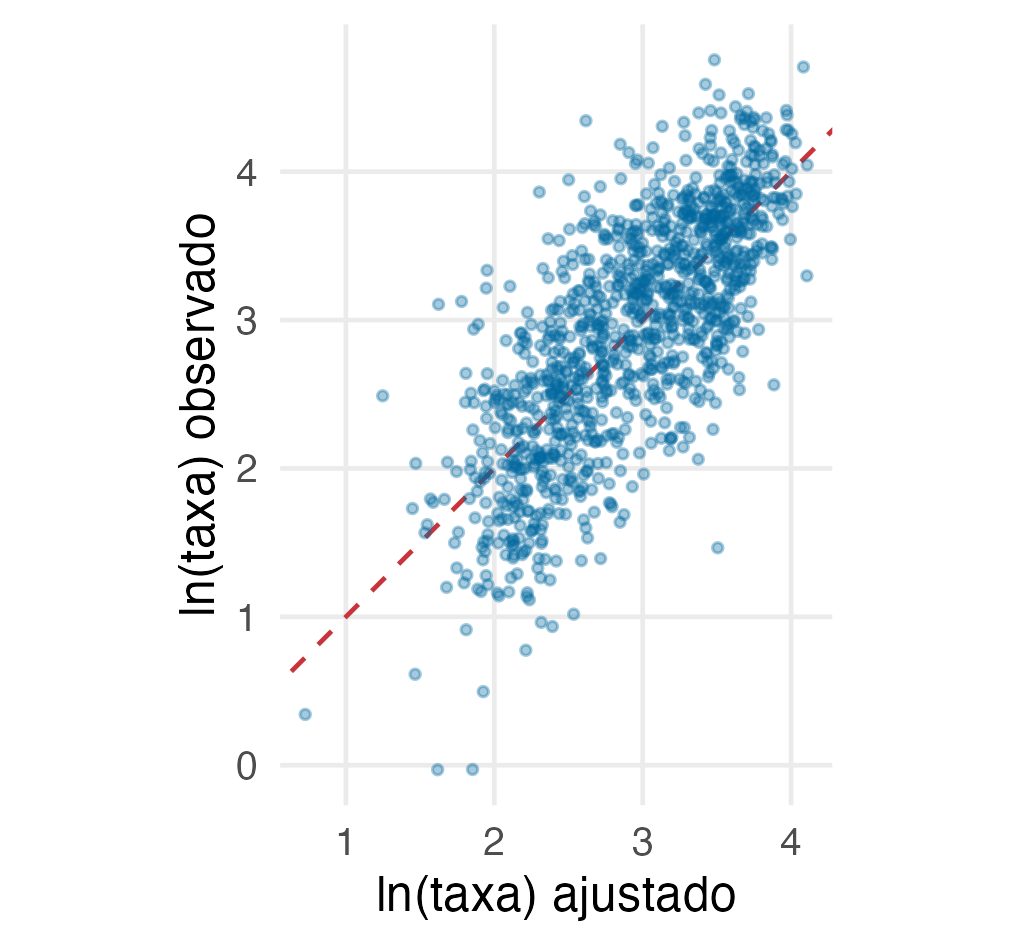
\includegraphics[width=0.55\textwidth]{observado_ajustado.png}
\caption{ln(taxa) observado contra ln(taxa) ajustado pelo modelo, nos mesmos dados do ajuste. A diagonal indica observado igual ao ajustado. \fonte}
\label{fig:ajuste}
\end{figure}

\subsection{Diagnóstico do modelo}
\label{sec:diag}

\textbf{Linearidade e variância.} Os resíduos contra os valores ajustados não mostram curva (Figura~\ref{fig:diag}, à esquerda). Nos resíduos contra cada explicativa, no caderno de análise, a curva suavizada fica perto de zero; só a distorção idade-série e o Gini mostram leve curvatura nos extremos, coerente com os quadrados significativos da Tabela~\ref{tab:espec}. A dispersão, porém, diminui nos municípios mais populosos (Figura~\ref{fig:diag}, à direita): a variância dos resíduos no quinto menos populoso é \nRazaoVar{} vez a do quinto mais populoso. Esse padrão é esperado, porque a taxa de um município pequeno se apoia em poucas mortes. O teste de Breusch-Pagan rejeita a variância constante ($BP = \nBP$, \nBPgl{} gl, $p$ \nBPp). Segundo a apostila, a heteroscedasticidade é uma violação menos grave: ela reduz a eficiência dos estimadores e invalida a estimativa da variância dos erros \citep[cap.~4]{ferrari2023}. Por isso, os intervalos e testes clássicos devem ser lidos com cautela.

\begin{figure}[htbp]
\centering
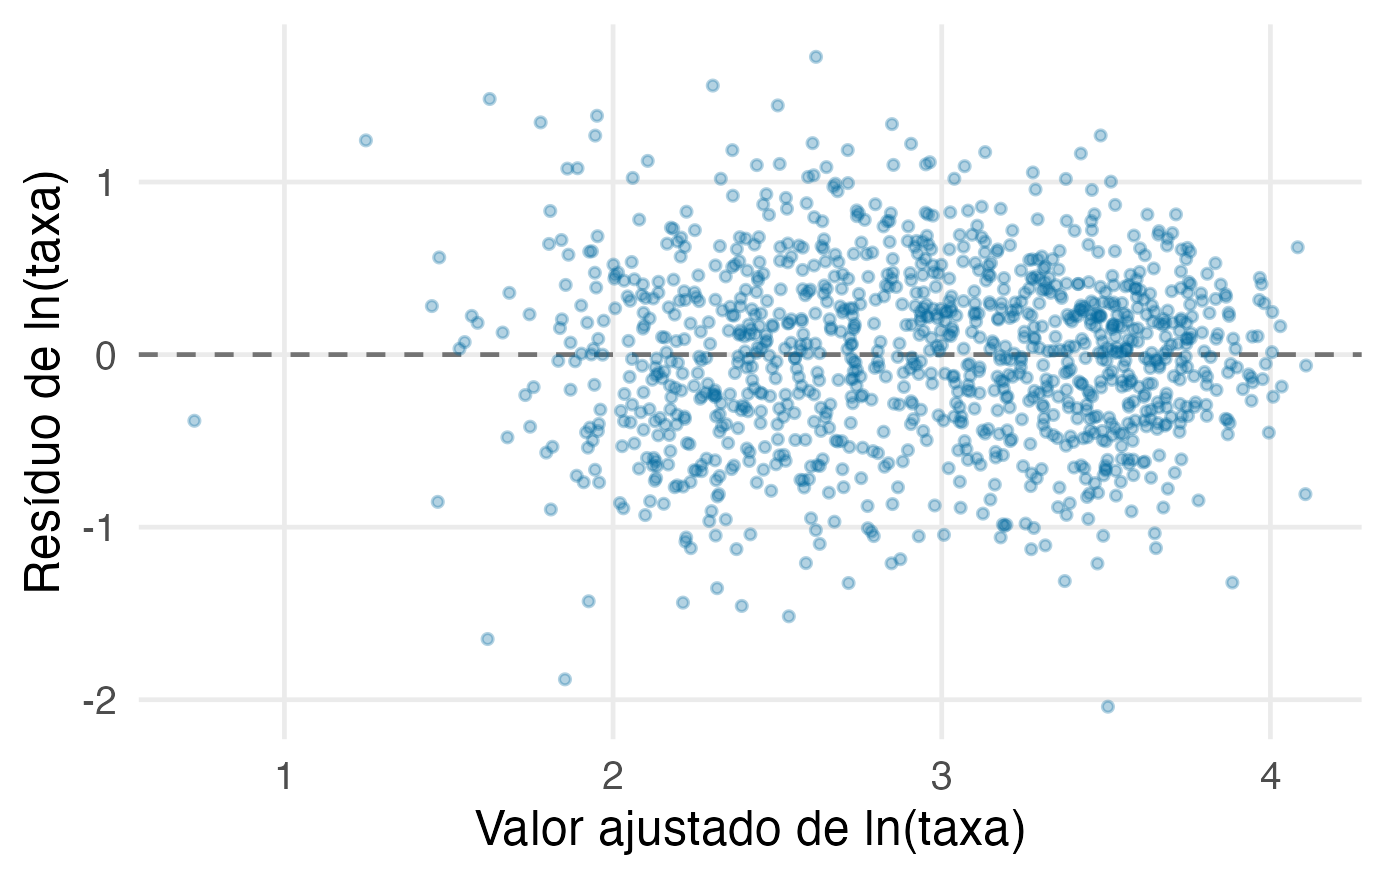
\includegraphics[width=0.48\textwidth]{residuos_ajustado.png}\hfill
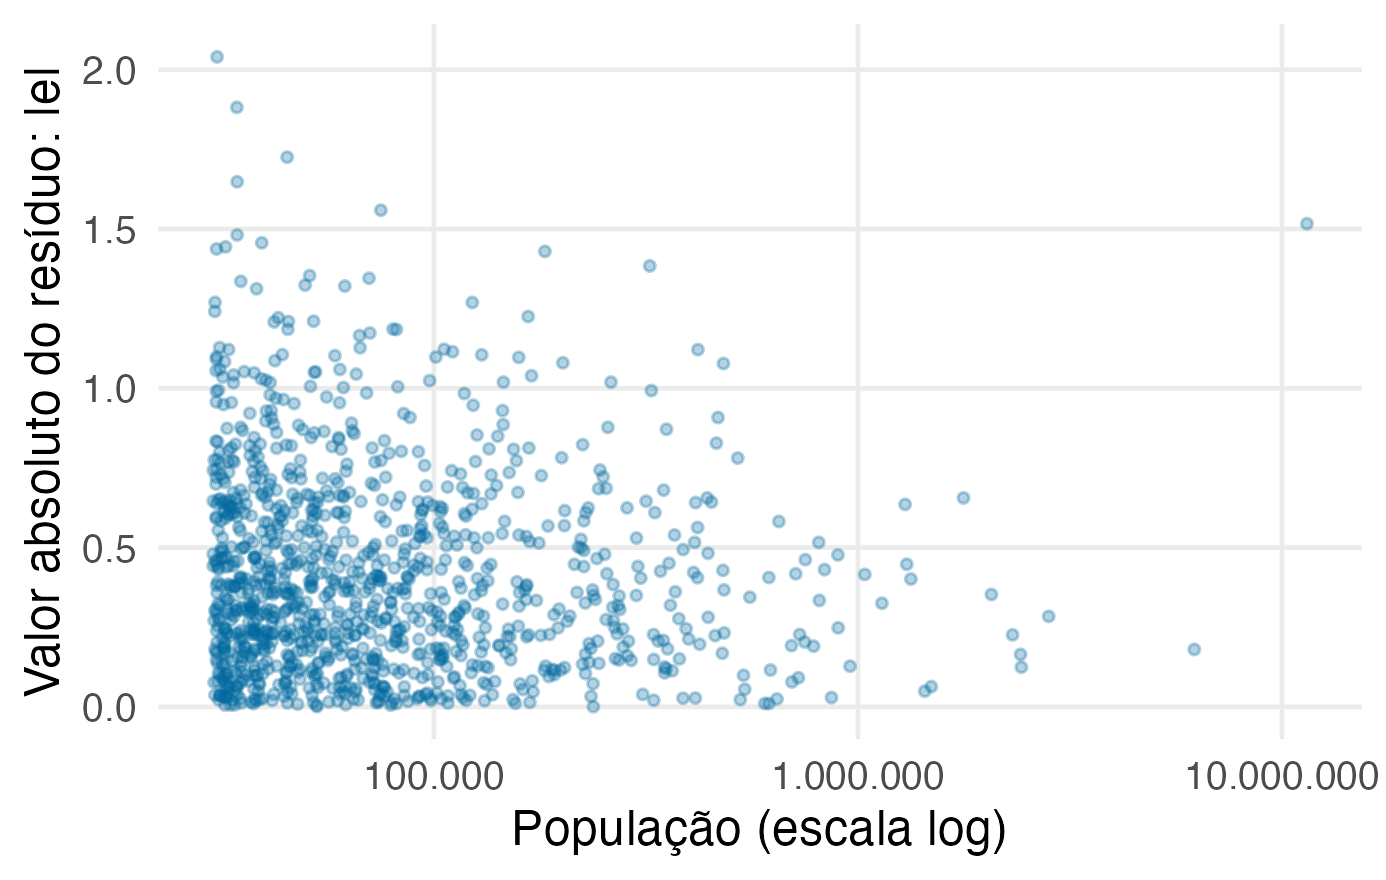
\includegraphics[width=0.48\textwidth]{residuos_populacao.png}
\caption{Esquerda: resíduos contra valores ajustados; a linha tracejada é o erro zero. Direita: tamanho do resíduo contra a população, em escala log. \fonte}
\label{fig:diag}
\end{figure}

\textbf{Medida corretiva.} A apostila indica mínimos quadrados ponderados (MQP) para a variância não constante, mas não define os pesos. Como escolha do grupo, aproximamos a variância de $\ln Y_i$ por $s_0^2 + 1/\mu_i$, em que $\mu_i$ é o número de homicídios esperado em três anos e $1/\mu_i$ é a parte da variância que vem do acaso da contagem; a parte restante foi estimada em $s_0^2 = \nSzeroQ$. Com pesos $1/(s_0^2 + 1/\mu_i)$, o coeficiente da interação passa de \nMqoInter{} para \nMqpInter, nenhum coeficiente troca de sinal, e o efeito de +0,05 no Gini nos percentis 10, 50 e 90 da renda fica em \nMqpGiniDez\%, \nMqpGiniCinq\% e \nMqpGiniNov\%. As estimativas e os sinais não dependem, portanto, da variância não constante. Mantivemos o MQO como modelo principal, por ser mais simples de interpretar.

\textbf{\textit{Outliers}, independência e normalidade.} Nenhum resíduo semi-studentizado atinge $\pm 4$; o maior, em valor absoluto, é \nMaxSemi. A independência espacial não foi verificada, como explicado na metodologia. Por último, no gráfico de quantis (Figura~\ref{fig:qq}), os pontos ficam próximos da reta. Pela regra empírica, \nRegraUm\%, \nRegraDois\% e \nRegraTres\% dos resíduos padronizados ficam a até 1, 1,645 e 1,96 desvios-padrão, contra 68\%, 90\% e 95\% esperados na normal. O Shapiro-Wilk não rejeita a normalidade ($W = \nSW$, $p = \nSWp$).

\begin{figure}[htbp]
\centering
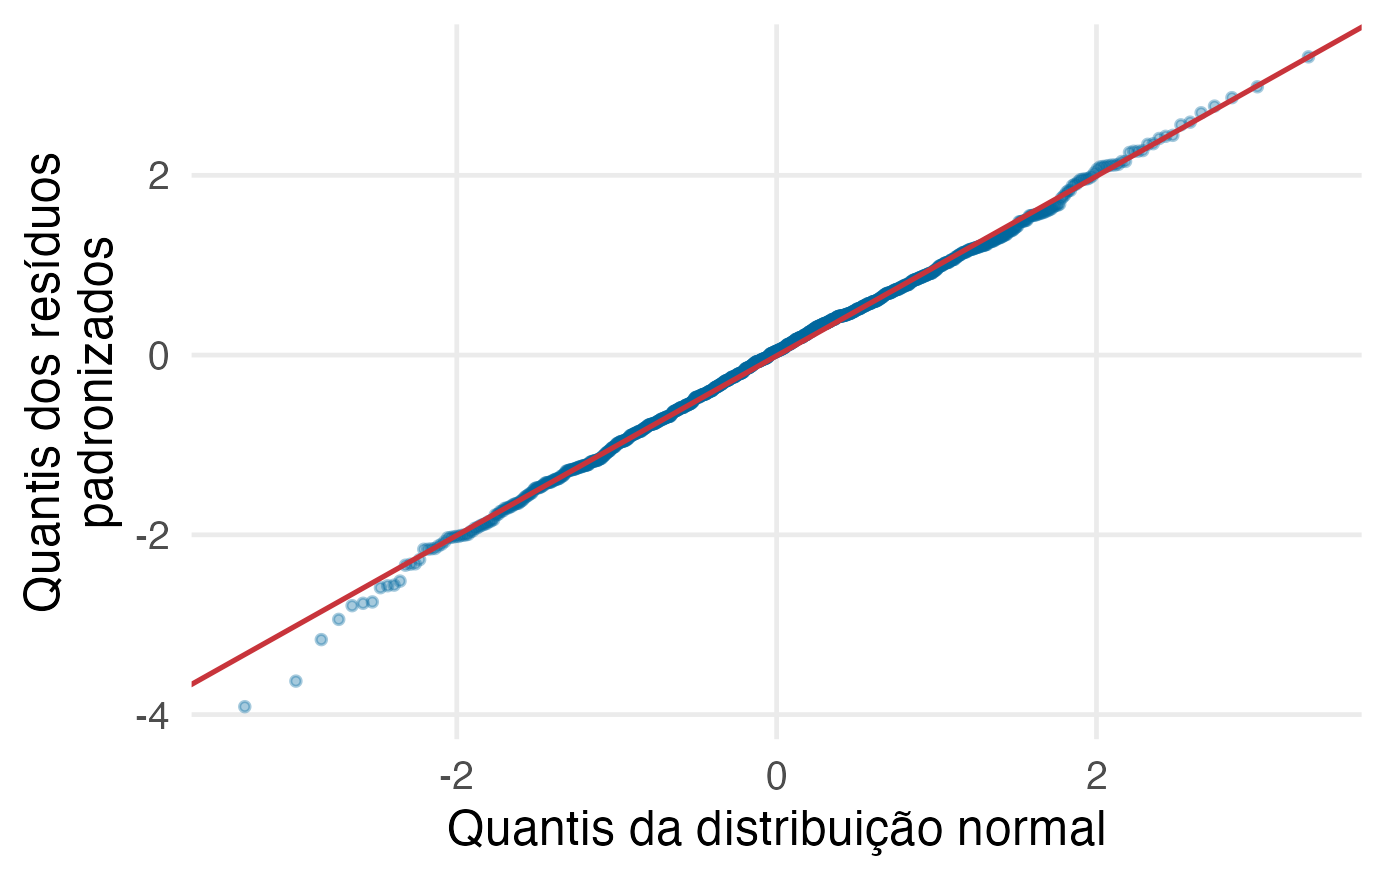
\includegraphics[width=0.50\textwidth]{qq_final.png}
\caption{Quantis dos resíduos padronizados contra quantis da distribuição normal. \fonte}
\label{fig:qq}
\end{figure}

\textbf{Multicolinearidade.} O maior VIF é \nVIFrendaFinal, da renda; o segundo maior é \nVIFsegundo, e o VIF médio é \nVIFmedio. Pelo critério da apostila, um VIF máximo de 5 ou 10 indica multicolinearidade, e um VIF médio maior que 1 também é indício do problema \citep[cap.~6]{ferrari2023}; os dois critérios apontam multicolinearidade. Ela não vem do termo quadrático (VIF \nVIFquad, após a centralização), mas da relação da renda com as demais explicativas: elas explicam \nRdoisRenda{} da variação da renda, que tem correlação de \nCorRendaUrbana{} com a urbanização. A multicolinearidade não impede o ajuste nem a previsão dentro do escopo, mas torna menos confiáveis os coeficientes isolados das variáveis correlacionadas com a renda. A apostila aponta ainda, como sinal de alerta, coeficientes com sinal contrário ao esperado. Três coeficientes têm sinal oposto ao da correlação simples (Tabela~\ref{tab:cor}): a desocupação, a urbanização e a migração, esta sem significância. Esses coeficientes são interpretados com cautela na próxima seção.

\subsection{Estimativas e interpretação}

A Tabela~\ref{tab:coef} traz os coeficientes, e a Tabela~\ref{tab:efeitos} traduz os principais em mudanças percentuais na taxa típica, com a hipótese de cada um na primeira coluna.

\begin{table}[htbp]
\centering
\caption{Coeficientes do modelo final. Resposta: $\ln Y$; $n = \nMunEsc$. Erros-padrão (EP) clássicos. \fonte}
\label{tab:coef}
\footnotesize
\setlength{\tabcolsep}{3pt}
\begin{tabular*}{\textwidth}{@{\extracolsep{\fill}}lrrrlrrr@{}}
\toprule
\textbf{Termo} & \textbf{$b$} & \textbf{EP} & \textbf{$p$} & \textbf{Termo} & \textbf{$b$} & \textbf{EP} & \textbf{$p$}\\
\midrule
Intercepto & 3,021 & 0,337 & $<$0,001 & Freq. escolar 15--17 & $-$0,018 & 0,004 & $<$0,001\\
ln(renda) centr. & $-$0,861 & 0,101 & $<$0,001 & Distorção EM & 0,014 & 0,002 & $<$0,001\\
(ln(renda) centr.)² & $-$0,998 & 0,092 & $<$0,001 & Migração recente & 0,004 & 0,003 & 0,143\\
Desigualdade (Gini, centr.) & 2,209 & 0,481 & $<$0,001 & Norte & 0,580 & 0,082 & $<$0,001\\
Gini $\times$ ln(renda) & 7,398 & 0,921 & $<$0,001 & Nordeste & 0,731 & 0,061 & $<$0,001\\
Desocupação & $-$0,018 & 0,008 & 0,022 & Centro-Oeste & 0,603 & 0,070 & $<$0,001\\
\% urbana & 0,011 & 0,002 & $<$0,001 & Sul & 0,515 & 0,055 & $<$0,001\\
\bottomrule
\end{tabular*}

\end{table}

\begin{table}[htbp]
\centering
\caption{Mudança percentual na taxa típica, com as demais variáveis constantes. O efeito do Gini está nos percentis 10, 50 e 90 da renda. O $p$ da renda é o do termo quadrático. IC 95\% clássico. \fonte}
\label{tab:efeitos}
\small
\begin{tabular}{@{}lrrcr@{}}
\toprule
 & \multicolumn{2}{c}{\textbf{Diferença}} & & \\
\cmidrule(lr){2-3}
\textbf{Variável} & \textbf{na explicativa} & \textbf{na taxa típica} & \textbf{IC 95\%} & \textbf{$p$}\\
\midrule
\multicolumn{5}{@{}l}{Hipóteses}\\
\quad H1: Gini (modelo sem a interação) & +0,05 & $+$16,2\% & [$+$10,9; $+$21,9] & $<$0,001\\
\quad H2: Distorção idade-série EM & +10 p.p. & $+$15,6\% & [$+$11,5; $+$19,8] & $<$0,001\\
\quad H2: Frequência escolar 15--17 & +5 p.p. & $-$8,6\% & [$-$11,9; $-$5,3] & $<$0,001\\
\quad H3: Migração recente & +5 p.p. & $+$2,1\% & [$-$0,7; $+$4,9] & 0,143\\
\addlinespace
\multicolumn{5}{@{}l}{Interação exploratória Gini $\times$ renda}\\
\quad Gini na renda de R\$ 699 & +0,05 & $-$10,0\% & [$-$16,8; $-$2,8] & 0,008\\
\quad Gini na renda de R\$ 1.383 & +0,05 & $+$15,8\% & [$+$10,6; $+$21,3] & $<$0,001\\
\quad Gini na renda de R\$ 2.043 & +0,05 & $+$33,7\% & [$+$26,3; $+$41,7] & $<$0,001\\
\addlinespace
\multicolumn{5}{@{}l}{Demais explicativas}\\
\quad Urbanização & +10 p.p. & $+$11,8\% & [$+$8,3; $+$15,4] & $<$0,001\\
\quad Desocupação & +1 p.p. & $-$1,8\% & [$-$3,3; $-$0,3] & 0,022\\
\bottomrule
\end{tabular}

\end{table}

\textbf{Desigualdade (H1).} A associação do Gini depende da renda (Figura~\ref{fig:gini}). Na renda mediana (R\$ \nRendaMediana), um aumento de 0,05 no Gini corresponde a uma taxa \nGiniEfMediana\% maior; no percentil 90 (R\$ \nRendaNoventa), a diferença chega a \nGiniEfNoventa\%. O efeito é zero perto de R\$ \nGiniZero{} per capita, e \nGiniZeroPct\% dos municípios ficam abaixo desse valor. No percentil 10 da renda (R\$ \nRendaDez), o efeito é negativo, de \nGiniEfDez\% ($p = \nGiniPDez$). H1 é, portanto, parcialmente sustentada: vale nos municípios de renda média e alta, mas não há um efeito positivo geral. Duas explicações possíveis, não testadas, são: nos municípios mais pobres, o Gini calculado por classes pode medir pior a desigualdade, porque muitas pessoas ficam nas classes mais baixas; e \nPctNEpobres\% dos municípios do décimo mais pobre estão no Nordeste, de modo que parte do efeito pode vir da região.

\begin{figure}[htbp]
\centering
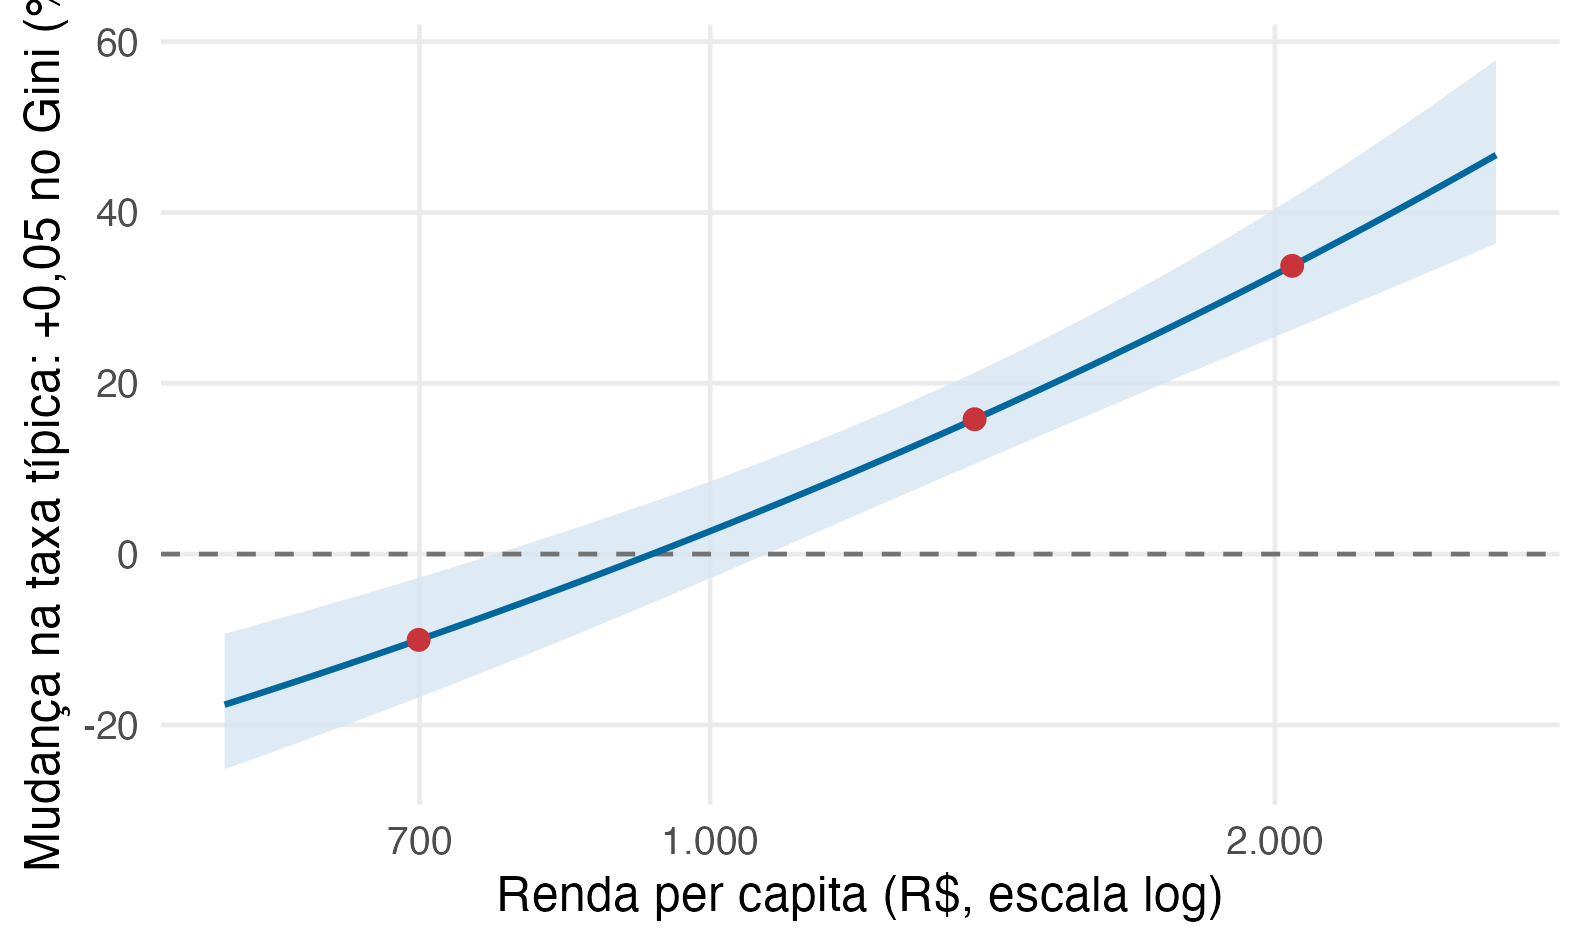
\includegraphics[width=0.62\textwidth]{gini_renda.png}
\caption{Mudança percentual na taxa típica para +0,05 no Gini, conforme a renda per capita. Faixa: IC 95\% clássico. Pontos: percentis 10, 50 e 90 da renda. \fonte}
\label{fig:gini}
\end{figure}

\textbf{Escola (H2).} As duas medidas escolares têm a direção esperada (Figura~\ref{fig:efeitos}). Cinco pontos percentuais a mais de frequência escolar de 15 a 17 anos correspondem a uma taxa \nEfFreq\% menor. Dez pontos a mais de distorção idade-série correspondem a uma taxa \nEfDist\% maior. H2 é sustentada. Essas medidas descrevem o município, e não o risco de cada jovem.

\textbf{Migração (H3).} Cinco pontos a mais de migração recente correspondem a uma taxa \nEfMigr\% maior, mas o intervalo de confiança inclui o zero ($p = \nPMigr$). H3 não é sustentada.

\textbf{Urbanização e desocupação.} Dez pontos a mais de população urbana correspondem a uma taxa \nEfUrb\% maior, como em \citet{wanzinack2022}, embora a correlação simples seja \nCorUrbana: o sinal só aparece com a renda no modelo, com a qual a urbanização tem correlação de \nCorRendaUrbana. A desocupação tem sinal negativo ($-$\nEfDesoc\% por ponto), embora a sua correlação simples com o logaritmo da taxa seja \nCorDesocup{} e a literatura aponte peso crescente do desemprego \citep{aransiola2021}. A desocupação tem correlação de \nCorDesocupRenda{} com a renda, e o coeficiente deixa de ser significativo a 5\% ao excluir os \nNSensDesoc{} municípios com 30\% ou mais de óbitos de intenção indeterminada entre os óbitos por causas externas ($p = \nPSensDesoc$). Não interpretamos esse coeficiente como efeito protetor.

\begin{figure}[htbp]
\centering
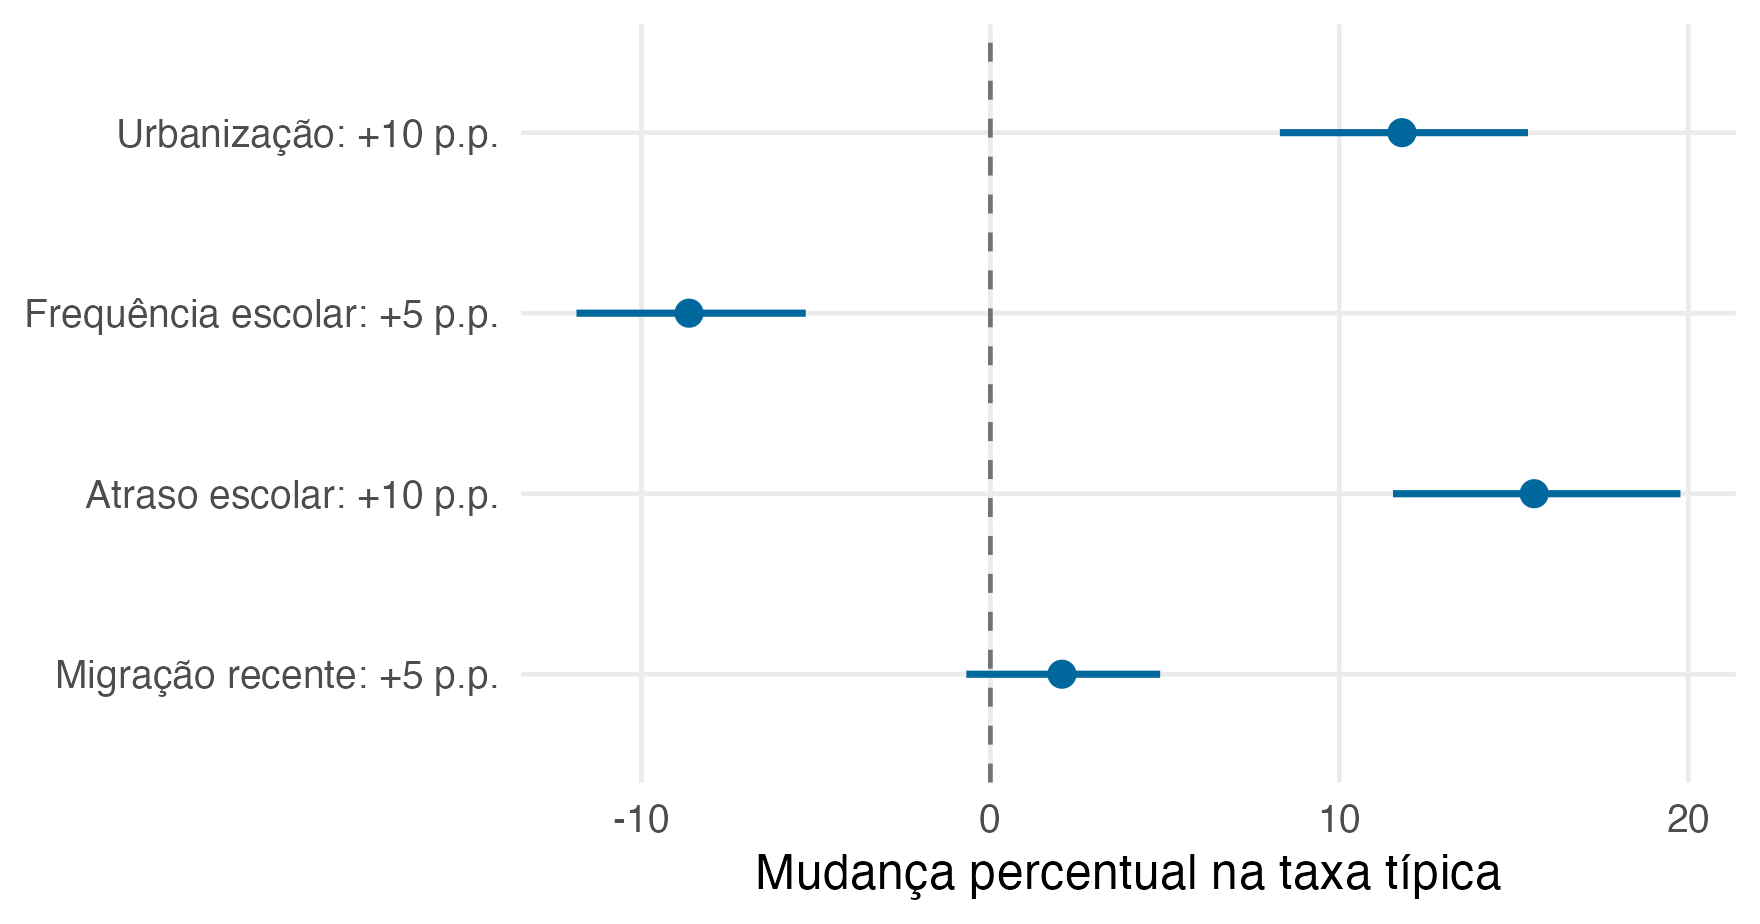
\includegraphics[width=0.62\textwidth]{efeitos.png}
\caption{Mudança percentual na taxa típica para as variáveis de escola, urbanização e migração. Barras: IC 95\% clássico; p.p. = pontos percentuais. \fonte}
\label{fig:efeitos}
\end{figure}

\textbf{Renda.} A relação com a renda tem forma de U invertido (Figura~\ref{fig:renda}), como a curva de Kuznets do crime \citep{buonanno2017} e o maior risco nas rendas intermediárias encontrado por \citet{duarte2012}. No Gini médio, a taxa típica ajustada é máxima perto de R\$ \nPico{} per capita e cai nos municípios mais ricos. Só \nPctAbaixoPico\% dos municípios ficam abaixo do pico; o trecho crescente da curva se apoia, portanto, em poucos casos. Por causa da interação, a posição do pico também muda com o Gini.

\textbf{Região.} Com as demais características iguais, todas as regiões têm taxa típica maior que o Sudeste: \nEfNE\% maior no Nordeste (IC 95\%: \nIcInfNordeste\% a \nIcSupNordeste\%), \nEfCO\% no Centro-Oeste (\nIcInfCentroOeste\% a \nIcSupCentroOeste\%), \nEfN\% no Norte (\nIcInfNorte\% a \nIcSupNorte\%) e \nEfS\% no Sul (\nIcInfSul\% a \nIcSupSul\%). O resultado do Sul chama atenção, pois a sua taxa bruta (\nTaxaSbr) é só um pouco maior que a do Sudeste (\nTaxaSEbr). Uma explicação provável é a referência: o Sudeste inclui São Paulo, a UF com a menor taxa do país em 2023 \citep{cerqueira2025}. A queda dos homicídios em São Paulo é atribuída a fatores como policiamento e controle de armas \citep{goertzel2009}, e a hipótese de que o PCC a explique não foi sustentada \citep{justus2018}. A região resume, portanto, fatores não medidos, como políticas estaduais de segurança e conflitos entre facções \citep{feltran2022}. Usamos a região, e não a UF, para manter poucos parâmetros: \nUFpoucos{} UFs têm menos de 10 municípios no estudo.

\begin{figure}[htbp]
\centering
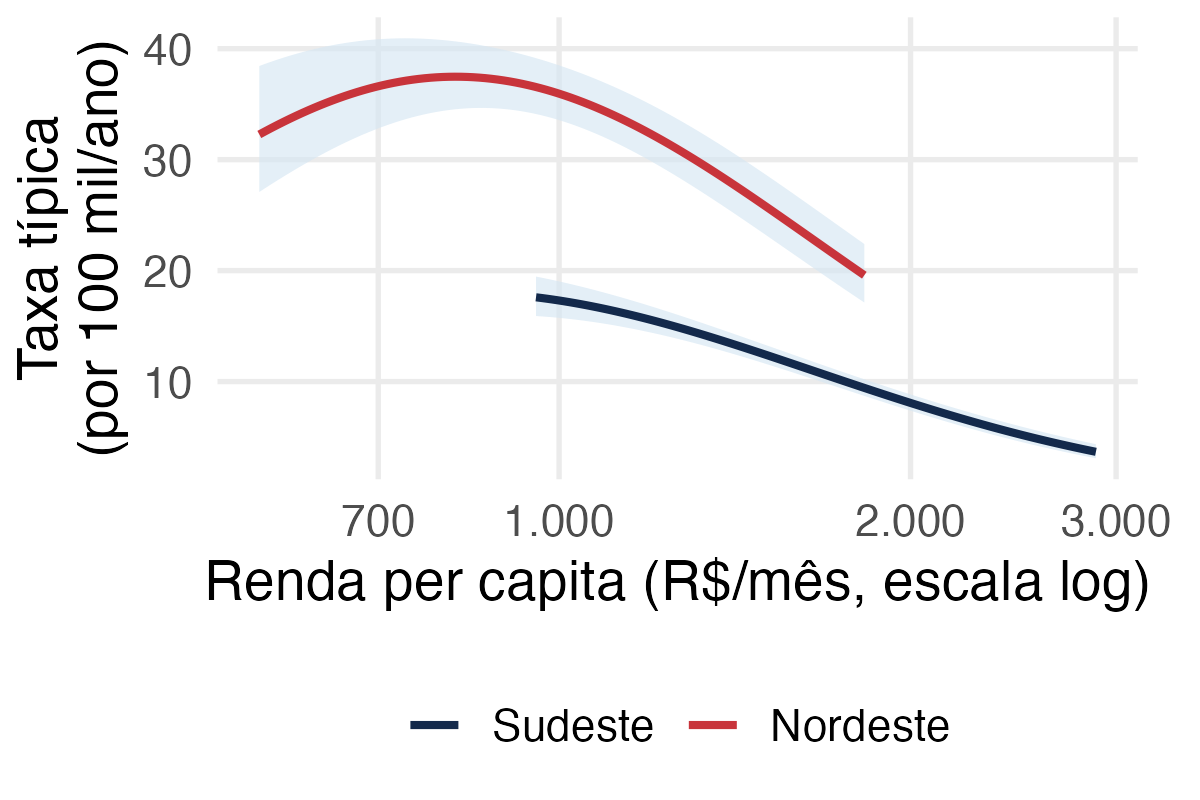
\includegraphics[width=0.62\textwidth]{renda_regiao.png}
\caption{Taxa típica ajustada conforme a renda per capita, no Nordeste e no Sudeste, no Gini médio e com as demais variáveis na média. Curvas no intervalo de renda observado em cada região. Faixas: IC 95\% clássico. \fonte}
\label{fig:renda}
\end{figure}

\subsection{Estimação e previsão}

A Tabela~\ref{tab:prev} aplica o modelo a um município típico, com cada explicativa na mediana do estudo, no Sudeste e no Nordeste. O intervalo de confiança refere-se à taxa típica de todos os municípios com essas características; o intervalo de previsão refere-se à taxa de um município. O intervalo de previsão é muito mais largo, porque soma a incerteza da estimativa à variação entre municípios. Como a variância não é constante, ele tende a ser largo demais para os municípios grandes e estreito demais para os pequenos. As previsões valem apenas dentro do escopo: municípios com 30 mil habitantes ou mais e combinações de características parecidas com as observadas.

\begin{table}[htbp]
\centering
\caption{Taxa típica estimada (por 100 mil ao ano) para um município com as explicativas na mediana do estudo. \fonte}
\label{tab:prev}
\small
\begin{tabular}{@{}lrccr@{}}
\toprule
\textbf{Região} & \textbf{Taxa típica} & \textbf{IC 95\%} & \textbf{IP 95\%} & \textbf{Mediana observada}\\
\midrule
Sudeste & 11,0 & [10,4; 11,6] & [3,9; 30,7] & 10,6\\
Nordeste & 33,3 & [31,5; 35,2] & [11,9; 93,1] & 35,8\\
\bottomrule
\end{tabular}

\end{table}

\subsection{Discussão}

Os resultados respondem à pergunta de pesquisa em três partes. Entre os fatores socioeconômicos, a renda tem relação curva com a taxa, e a desigualdade se associa a taxas maiores sobretudo nos municípios de renda média e alta. Entre os fatores educacionais e demográficos, a frequência e o atraso escolar têm as associações esperadas, a urbanização associa-se a taxas maiores e a migração recente não mostrou associação clara. Entre os fatores geográficos, as diferenças regionais permanecem com as demais características iguais.

O resultado central é a interação entre Gini e renda. Um estudo com todos os municípios brasileiros estimou um único efeito do Gini \citep{wanzinack2022}; no nosso modelo, esse efeito médio esconde sinais opostos nos extremos da renda. O resultado é coerente com estudos entre países, nos quais a desigualdade pesa mais em níveis intermediários de desenvolvimento \citep{ouimet2012} e condiciona o efeito da renda \citep{aransiola2024}. O grupo esperava um efeito único da desigualdade (H1); os dados mostraram que a pergunta relevante é para quais municípios a desigualdade importa.

Como pontos positivos, o trabalho usa o Gini municipal do Censo 2022, validado nas UFs; reduz o ruído das taxas com a média de três anos e o recorte por porte; constrói o modelo em blocos testados pelo $F$ parcial e confirmados por MSE, AIC, BIC e PRESS; diagnostica o modelo antes de interpretar os coeficientes; e confirma as conclusões com o ajuste ponderado. Como pontos negativos, a variância não é constante, o logaritmo não é a potência ótima do Box-Cox, o Gini é aproximado, o sinal da desocupação não tem explicação clara, termos adicionais significativos ficaram fora por parcimônia e a região absorve fatores que o modelo não mede.

\section{Considerações Finais}

Este trabalho identificou as características municipais associadas à taxa de homicídios no Brasil, com um modelo de regressão linear múltipla para \nMunEsc{} municípios com 30 mil habitantes ou mais, que reúnem \nPctPopEsc\% da população. O modelo explica \nRdoisPct\% da variação do logaritmo da taxa. A desigualdade associa-se a taxas maiores nos municípios de renda média e alta (H1 parcialmente sustentada). A exclusão escolar associa-se a taxas maiores (H2 sustentada). A migração recente não mostrou associação clara (H3 não sustentada). A renda tem relação em U invertido com a taxa, e as regiões Norte, Nordeste, Centro-Oeste e Sul têm taxas típicas maiores que o Sudeste. Esses resultados são associações entre municípios: eles não demonstram causa nem descrevem o risco de cada pessoa. Para a meta 16.1 do ODS 16, eles sugerem que políticas de permanência escolar e de redução da desigualdade nos municípios de renda média e alta merecem atenção, a ser confirmada por estudos causais.

\subsection{Limitações}

\begin{itemize}
\item \textbf{Variância não constante.} O Breusch-Pagan rejeita a variância constante. O ajuste ponderado mantém as conclusões, mas os intervalos e testes clássicos devem ser lidos com cautela.
\item \textbf{Vizinhança.} Municípios próximos podem compartilhar fatores não medidos. A independência dos erros no espaço não foi verificada, a pedido da professora; erros correlacionados exigem modelos que estão fora do escopo da apostila.
\item \textbf{Medição.} O Gini é uma aproximação pelas classes de renda. O SIM pode omitir ou classificar mortes de forma diferente entre municípios. Os municípios com menos de 30 mil habitantes ficaram fora, e os resultados não se aplicam diretamente a eles.
\item \textbf{Especificação.} Quatro dos cinco conjuntos de termos adicionais da Tabela~\ref{tab:espec} são significativos, mas ficaram fora por parcimônia. O coeficiente da desocupação é frágil.
\item \textbf{Estudo observacional.} Os dados são de um único período, e fatores como policiamento e crime organizado não foram medidos.
\end{itemize}

\textbf{Trabalhos futuros.} O estudo pode ser ampliado de quatro formas: (1) investigar a dependência espacial entre municípios vizinhos; (2) testar se a interação entre Gini e renda e a curva da renda diferem entre regiões; (3) incluir dados de políticas estaduais de segurança e de violência organizada; (4) acompanhar os municípios em vários anos, para separar diferenças permanentes de mudanças no tempo.

\bibliographystyle{sbpo}
\bibliography{referencias}

\end{document}
